\documentclass{standalone}
\usepackage{tikz}
\usetikzlibrary{patterns}
\usetikzlibrary{decorations.pathmorphing}
\begin{document}
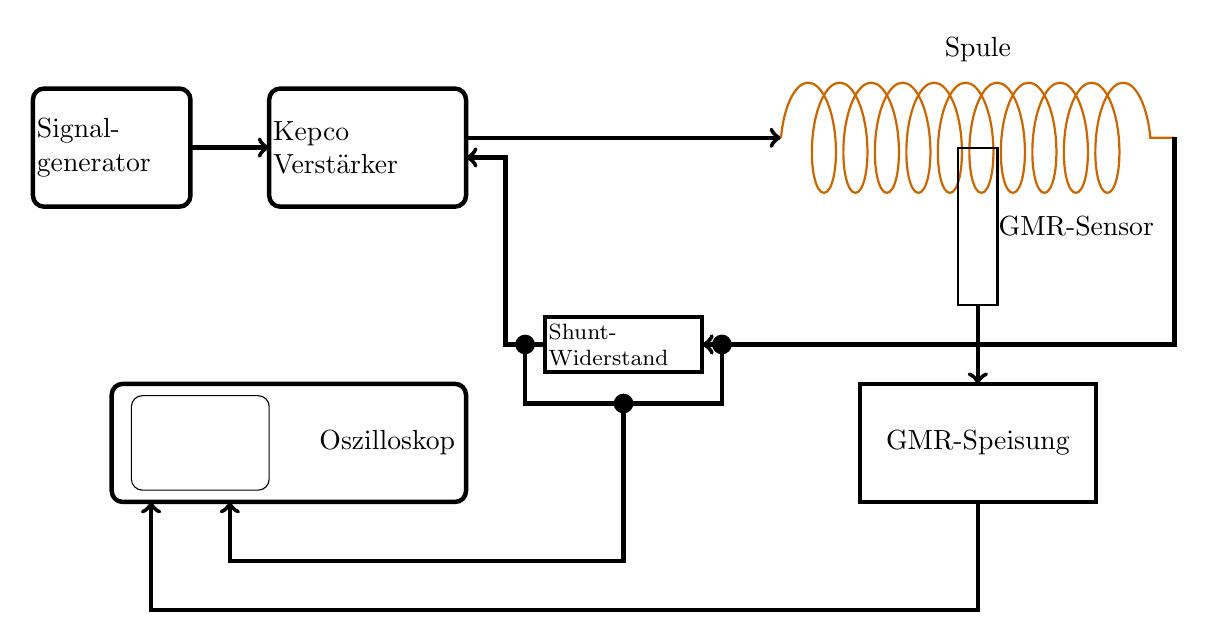
\begin{tikzpicture}
    %\fill[black,opacity = 0.6,rounded corners] (1,1) rectangle (1.6,1.8);


    %\draw[decoration={aspect=0.3, segment length=3mm, amplitude=3mm,coil},decorate] (0,5) -- (0,10);



    \draw[black,ultra thick,rounded corners] (0,0) rectangle (2,1.5);
    \node at (1,.75) {\parbox{1.9cm}{Signal-\\generator}};

    \draw[->,ultra thick] (2,.75) -- (3,.75);
    \draw[black,ultra thick,rounded corners] (3,0) rectangle (5.5,1.5);
    \node at (4,.75) {\parbox{1.9cm}{Kepco \\ Verst\"arker}};

    \draw[->,ultra thick] (5.5,.75+.125) -- (9.5,.75+.125);
    \draw[thick,color=orange!80!black,decoration={aspect=0.35, segment length=4mm, amplitude=7mm,coil},decorate] (9.5,.75+.125) -- (14.5,.75+.125);
    \node at (12,2) {Spule};

    \draw[->,ultra thick] (14.5,.76+.125) -- (14.5,-1.75) -- (8.5,-1.75);
    \draw[black,ultra thick] (6.5,-1.75+.7/2) rectangle (8.5,-1.75-.7/2);
    \node at (7.5,-1.75) {\footnotesize\parbox{1.9cm}{Shunt-Widerstand}};

    % line from shunt resistor to amplifier
    \draw[->,ultra thick] (6.5,-1.75) -- (6,-1.75) -- (6,.75-.125) -- (5.5,.75-.125);

    % GMR sensor
    \draw[black,thick] (11.75,0.75) rectangle (12.25,-1.25);
    \node at (13.25,-0.25) {GMR-Sensor};

    % line from GMR sensor to GMR box
    \draw[->,ultra thick] (12,.-1.25) -- (12,-2.25);

    % GMR box
    \draw[black,ultra thick] (13.5,-2.25) rectangle (10.5,-3.75);
    \node at (12,-3) {GMR-Speisung};

    %\draw[->,ultra thick] (10.5,.-3) -- (5.5,-3);

    % line from GMR box to oscilloscope
    \draw[->,ultra thick] (12,-3.75) -- (12,-5-.125) -- (1.5,-5-.125) -- (1.5,-3.75);
    %\draw[->,ultra thick] (12+.125,-3.75) -- (12+.125,-5-.125) -- (1.5-.125,-5-.125) -- (1.5-.125,-3.75);
    %\draw[->,ultra thick] (12-.125,-3.75) -- (12-.125,-5+.125) -- (1.5+.125,-5+.125) -- (1.5+.125,-3.75);

    % oscilloscpe
    \draw[black,ultra thick,rounded corners] (5.5,-2.25) rectangle (1,-3.75);
    \draw[black,rounded corners] (3,-2.4) rectangle (1.25,-3.6);
    \node at (4.5,-3) {Oszilloskop};

    % Measurement of shunt voltage
    %\draw[->,ultra thick] (6.25,-1.75) -- (6.25,-2.5) -- (7.5-.125,-2.5) -- (7.5-.125,-4.25) -- (2.75,-4.25) -- (2.75,-3.75);
    %\draw[->,ultra thick] (8.75,-1.75) -- (8.75,-2.5) -- (7.5+.125,-2.5) -- (7.5+.125,-4.5)  -- (2.5,-4.5) -- (2.5,-3.75);
    \draw[-,ultra thick] (6.25,-1.75) -- (6.25,-2.5) -- (7.5-.125,-2.5);
    \draw[-,ultra thick] (8.75,-1.75) -- (8.75,-2.5) -- (7.5+.125,-2.5);
    \fill (7.5,-2.5) circle [radius=0.125];
    \draw[->,ultra thick] (7.5,-2.5) -- (7.5,-4.5)  -- (2.5,-4.5) -- (2.5,-3.75);
    \draw[-,ultra thick] (6.25 - 0.025,-2.5) -- (8.75 + 0.025,-2.5);
    \fill (6.25,-1.75) circle [radius=0.125];
    \fill (8.75,-1.75) circle [radius=0.125];
    %\draw[black,ultra thick] (6.5,-1.75+.7/2) rectangle (8.5,-1.75-.7/2);
\end{tikzpicture}
\end{document}
